\documentclass{SBCbookchapter}

% Fontes
\usepackage[utf8]{inputenc}
\usepackage[T1]{fontenc}

% Língua
\usepackage[brazilian]{babel}

% Figuras
\usepackage{graphicx}
\graphicspath{{img/}}

% Referências
\usepackage[brazilian]{backref}
\usepackage[alf]{abntex2cite}

% Serpa

\usepackage{booktabs} 
\usepackage{tikz}
\usepackage{listings,xcolor}
\usepackage[framed,numbered,autolinebreaks,useliterate]{mcode}

\newcounter{chapter}\setcounter{chapter}{1}

\author{\textbf{Matheus da Silva Serpa}\\ \textit{msserpa@inf.ufrgs.br}\\ \textit{Grupo de Processamento Paralelo e Distribuído (GPPD) \\ Universidade Federal do Rio Grande do Sul (UFRGS) \\ Sala 201, Av. Bento Gonçalves, 9500 - Campus do Vale\\ 91.501-970 - Porto Alegre - RS - Brasil}\\~\\
\textbf{Philippe Olivier Alexandre Navaux}\\ \textit{navaux@inf.ufrgs.br}\\ \textit{Grupo de Processamento Paralelo e Distribuído (GPPD) \\ Universidade Federal do Rio Grande do Sul (UFRGS) \\ Sala 210, Av. Bento Gonçalves, 9500 - Campus do Vale\\ 91.501-970 - Porto Alegre - RS - Brasil}\\~\\
\textbf{Jairo Panetta}\\ \textit{jairo.panetta@gmail.com}\\ \textit{Divisão de Ciência da Computação (IEC) \\ Instituto Tecnológico de Aeronáutica (ITA) \\ Sala 109, Praça Marechal Eduardo Gomes, 50 - Vila das Acácias \\ 12228-900 - São José dos Campos - SP - Brasil} } 


\title{Programação com Aceleradores Vetoriais}

\definecolor{mygreen}{RGB}{2,112,10}

\newlength\listingnumberwidth
\setlength\listingnumberwidth{10pt}
\lstset{
  showstringspaces=false,
  language=C,
  escapeinside={@}{@},
  basicstyle=\small\ttfamily,
  numbersep=5pt,
  breaklines=true
}

\newcommand{\ms}[1]{\textcolor{red}{\textbf{msserpa: #1} }}

\begin{document}
\maketitle

\begin{resumo}
Tradicionalmente, o aumento de desempenho das aplicações se dava de forma transparente aos programadores através do aumento do paralelismo a nível de instruções e do aumento de frequência dos processadores. Entretanto, esse modelo não se sustenta mais. Para se ganhar desempenho nas arquiteturas modernas, são necessários conhecimentos sobre programação paralela e vetorial. Ambos paradigmas são tratados de forma lateral em cursos de computação, sendo que muitas vezes nem são abordados. Nesse contexto, este capítulo objetiva propiciar um maior entendimento sobre os paradigmas de programação paralela e vetorial, de forma que os participantes aprendam a otimizar adequadamente suas aplicações para arquiteturas modernas. Como plataforma experimental, será utilizado o processador vetorial NEC SX-Aurora TSUBASA. Será enfatizada a importância do processamento vetorial e de matrizes, presente em várias aplicações, tais como de petróleo e na área de previsões climáticas.
\end{resumo}
\section{Introdução}

A introdução de circuitos integrados, \textit{pipelines}, aumento da frequência das operações, execução fora de ordem e previsão de desvios constituem parte importante das tecnologias introduzidas até o final do século XX. Recentemente, tem crescido a preocupação com o consumo energético, com o objetivo de se atingir a computação em nível \textit{exascale} de forma sustentável. Entretanto, as tecnologias até então desenvolvidas não possibilitam atingir tal fim, devido ao alto custo energético de se aumentar a frequência e estágios de \textit{pipeline}, assim como a chegada nos limites de exploração do paralelismo a nível de instrução~\cite{borkar2011future,coteus2011technologies}. 

Este capítulo envolve o estudo de aspectos relacionados à arquitetura de computadores e a elaboração, execução e teste de programas concorrentes. Neste sentido, pretende-se inicialmente identificar as arquiteturas de \textit{hardware} que existem atualmente e que podem ser utilizadas para a construção de máquinas de alto desempenho. Em um segundo momento, a interface de programação OpenMP será apresentada para ambientes de memória compartilhada. Com base nesta interface, almeja-se elaborar aplicações paralelas otimizadas. 

Para os programas a serem desenvolvidos são disponibilizados códigos fonte sequenciais e paralelos previamente criados e testados.  Os exemplos de código serão introduzido de forma incremental, isto é, variações do mesmo código serão fornecidas para testar aspectos distintos oferecidos pelas interfaces de programação. Por fim, alguns tópicos de testes, depuração e medição de desempenho serão citadas, com o intuito de mostrar como são feitas avaliações de performance de aplicações paralelas.

A estrutura do capítulo é dividida em 7 partes. Inicialmente será apresentada uma introdução sobre as arquiteturas paralelas na Seção~\ref{sec:arquitetura}. Na sequência será explicitado, na Seção~\ref{sec:modelagem}, como pode ser feita a modelagem de aplicações paralelas. A Seção~\ref{sec:openmp} discute como se pode programar paralelamente uma arquitetura de memória compartilhada usando a biblioteca de diretivas OpenMP. Essa seção também aborda a programação vetorial usando instruções SIMD. A avaliação de desempenho com contadores de \textit{hardware} do tipo Linux perf e Performance Application Programming Interface (PAPI) é apresentada na Seção~\ref{sec:contadores}. 
A Seção~\ref{sec:experiments} mostra um estudo de caso sobre o desempenho de uma aplicação de geofísica utilizando os conceitos apresentados no capítulo e, finalmente, a Seção~\ref{sec:conclusion}, traz-se a conclusão, abordando as potencialidades de paralelismo com outras interfaces de programação.
\section{Arquiteturas Paralelas}\label{sec:arquitetura}

Algumas das primeiras perguntas a serem feitas em relação ao desenvolvimento de aplicações é: por que estudar programação paralela?, os programas já não são rápidos o suficiente? as máquinas já não são rápidas o suficiente? Um dos principais pontos de motivação é que os requisitos necessários estão sempre mudando. Os usuários desejam executar aplicações e jogos cada vez mais detalhistas e com tempo de resposta menor. Além de que, desde 2005, é difícil encontrar um processador de um só \textit{core} no mercado~\cite{fruehe2005multicore, gepner2006multi}.

Outros motivos para utilizar programação paralela são: (i) reduzir o tempo necessário para solucionar um problema e (ii) resolver problemas mais complexos e de maior dimensão em um tempo aceitável. Existem além desses, outros motivos como: utilizar recursos computacionais subaproveitados; ultrapassar limitações de memória quando a memória disponível num único computador é insuficiente para a resolução do problema; e também ultrapassar os limites físicos que atualmente começam a restringir a possibilidade de construção de computadores sequenciais cada vez mais rápidos.

Nesse sentido, a computação de alto desempenho tem sido responsável por uma revolução científica. A evolução das arquiteturas de computadores melhorou o poder computacional, aumentando a gama de problemas e a qualidade das soluções que poderiam ser resolvidas no tempo requerido como, por exemplo, a previsão do tempo. Entretanto, devido a limitações de consumo de energia, dissipação de calor, dimensão do processador e uma melhor distribuição das \textit{threads} para processamento, a indústria mudou seu foco para arquiteturas paralelas e sistemas distribuídas~\cite{hsu2015three,borkar2011future,coteus2011technologies}.

A principal característica dessas arquiteturas é a presença de vários núcleos de processamento operando simultaneamente. No entanto, o desenvolvimento de \textit{software} foi afetado por essa mudança de paradigma e diversas aplicações sofreram reengenharias para tornar possível o aproveitamento dos recursos através da execução paralela~\cite{Gropp2013,Mittal2015,Cruz2016}.

\subsection{Classificação de Arquiteturas Paralelas}

A classificação de Flynn~\cite{flynn1996parallel} baseia-se no fato de um computador executar uma sequência de instruções sobre uma sequência de dados. As instruções e os dados são separados em um ou vários fluxos de instruções (\textit{instruction stream}) e um ou vários fluxos de dados (\textit{data stream}). Essa classificação possui quatro classes, mas vamos nos concentrar apenas nas duas classes que representam as arquiteturas paralelas: \textit{Single Instruction Multiple Data} (SIMD) e \textit{Multiple Instruction Multiple Data} (MIMD). A Figura~\ref{fig:simd_mimd} apresenta os diagramas das classes exemplificadas a seguir.

\begin{figure}[!htb]
	\centering
	\caption{Diagramas das classes SIMD (esquerda) e MIMD (direita).}
	\label{fig:simd_mimd}
	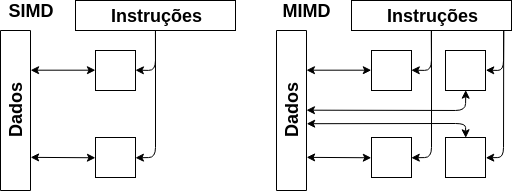
\includegraphics[scale=0.6]{flynn.png}
\end{figure}

Em uma arquitetura SIMD, uma única instrução é executada ao mesmo tempo sobre múltiplos dados. Esse processamento é controlado por uma única unidade de controle que é alimentada por um único fluxo de instruções. Cada instrução é enviada para todos processadores que executam as instruções em paralelo de forma síncrona sobre diferentes fluxos de dados. Essa arquitetura é encontrada nas unidades MMX/SSE de processadores \textit{multicore} e nas \textit{Graphics Processing Units} (GPUs).

Em arquiteturas MIMD, cada unidade de controle recebe um fluxo de instruções próprio e repassa-o para seu respectivo processador. Dessa forma, cada processador executa suas instruções em seus dados de forma assíncrona. O princípio dessa classe é bastante genérico, pois se um computador de um grupo de máquinas for analisado separadamente, este pode ser considerado uma máquina MIMD. Nessa classe encontram-se as arquiteturas paralelas \textit{multicore}.

Arquiteturas paralelas atuais combinam ambas arquiteturas SIMD e MIMD. Por exemplo, um processador \textit{multicore} possui vários \textit{cores} cada um trabalhando sobre um conjunto de instruções e um conjunto de dados, ou seja, MIMD. Em cada \textit{core} do mesmo processador existe uma unidade especial de ponto flutuante que explora SIMD. Sistemas distribuídos são compostos por várias arquiteturas paralelas, logo, combinando SIMD e MIMD.

\subsection{Arquiteturas Multicore e Manycore}

Desde 2003, a indústria vem seguindo duas abordagens para o projeto de microprocessadores~\cite{kirk2016programming}. A abordagem multicore é orientada à latência, onde instruções são executadas em poucos ciclos de \textit{clock}. Por outro lado, as arquiteturas manycore tem uma abordagem focada ao \textit{throughput}, ou seja, um grande número de instruções é executado por unidade de tempo.

O projeto das arquiteturas multicore e manycore é diferente ao ponto que dependendo da aplicação, o desempenho pode ser muito grande em uma arquitetura e muito pequeno na outra~\cite{cook2012cuda}. A arquitetura multicore utiliza uma lógica de controle sofisticada para permitir que instruções de uma única \textit{thread} sejam executadas em paralelo. Grandes memórias \textit{cache} são fornecidas para reduzir latências de acesso às instruções e dados de aplicações que tem acesso à memória predominante. Por fim, as operações das Unidades Lógicas e Aritméticas (ULA) também são projetadas visando otimizar a latência.

A arquitetura manycore tira proveito de um grande número de \textit{threads} de execução. Pequenas memórias \textit{cache} são fornecidas para evitar que múltiplas \textit{threads}, acessando os mesmos dados, precisem ir até a memória principal. Além disso, a maior parte do \textit{chip} é dedicada a unidades de ponto flutuante. Arquiteturas desse tipo são projetadas como mecanismos de cálculo de ponto flutuante e não para operações convencionais, que são realizadas por arquiteturas multicore. Algumas aplicações poderão utilizar tanto multicore quanto manycore em conjunto, sendo cada arquitetura melhor para um tipo de operação.
\section{Modelagem de Aplicações Paralelas} \label{sec:modelagem}

A programação paralela possibilita utilizar ao máximo os recursos de \textit{hardware}. Com isso, muitos problemas antes impossíveis de serem solucionados podem ser executados sem muito esforço. A demanda de desempenho necessária para a realização de uma tarefa está relacionada com a quantidade de dados ou variáveis envolvidas durante o processamento e quais as operações pelas quais estes terão de passar até o resultado. Quanto mais eficiente for a implementação de um algoritmo, menor a demanda por desempenho.

Segundo Foster~\cite{foster1995designing}, a modelagem de um problema de forma paralela passa por quatro fases: o particionamento, a comunicação, o agrupamento e o escalonamento.

\begin{description}
\item[1) Particionamento] - Primeiramente, os dados são divididos de maneira que cada tarefa possa ser executada independentemente das demais. Com isso obtém-se a menor granularidade possível para cada tarefa.

\item[2) Comunicação] - Em um segundo momento, devido ao fato de os dados normalmente estarem inter-relacionados, é necessário que haja a troca de informações entre os processos. Nessa fase é definida a forma de comunicação paralela adotada, caso seja utilizado uma arquitetura multiprocessada.

\item[3) Agrupamento] - Em seguida, em uma terceira fase, as operações ou dados são agrupados a fim de realizar um melhor uso dos processadores. O objetivo dessa fase é aumentar a granularidade das operações realizadas por um único processador. Assim, operações que envolvam um conjunto de dados vizinho são executadas em um mesmo processador, diminuindo a interdependência entre os dados.

\item[4) Escalonamento] - Por fim, na quarta etapa, ocorre o mapeamento, que é a fase que define como serão distribuídas as tarefas entre os processadores. Essa distribuição busca casar a granularidade das tarefas com a capacidade de processamento dos processadores e a dependência entre os processos que se encontram em processadores distintos.

\end{description}

A Figura~\ref{fig:modelagemFoster} ilustra cada uma das etapas descritas anteriormente. Inicialmente um conjunto de dados é particionado. Posteriormente são destacadas as interações entre dois pontos vizinhos de granularidade fina. Após o agrupamento entre alguns pontos é feito um mapeamento, que distribui as tarefas entre 5 processadores ($P1,...,P5$).


\begin{figure}[!htbp]
	\centerline{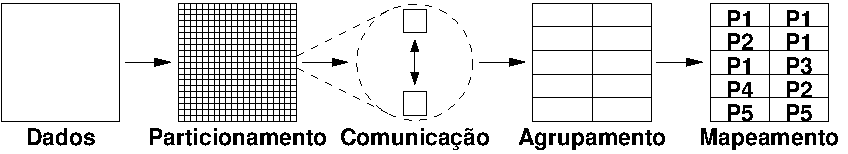
\includegraphics[scale=1.0]{modelagemFoster}}
	\caption{Principais etapas na paralelização de um algoritmo.}
	\label{fig:modelagemFoster}
\end{figure}

Mais conceitos de projeto e desenvolvimento de programas paralelos podem ser estudados no material base do minicurso Projetando e Construindo Programas Paralelos, apresentando na ERAD/RS 2019\footnote{https://www.setrem.com.br/erad2019/data/pdf/minicursos/mc02.pdf}.
\section{Programação Paralela e Vetorial em OpenMP}\label{sec:openmp}

Os modelos de programação paralela são divididos em modelos de memória compartilha e de memória distribuída. Exemplos de modelos de programação em memória compartilhada são OpenMP (\emph{Open Multi-Processing})~\cite{openmp,chapman2008using}, Cilk~\cite{reinders2012overview,robison2013composable} e CUDA (\emph{Compute Unified Device Architecture})~\cite{cook2012cuda,kirk2016programming}. Nesse ambiente, a programação é feita utilizando \textit{threads}. A decomposição utilizada é na sua maioria a decomposição do domínio ou a funcional, com diferentes granularidades. No caso dos modelos de memória distribuída, o MPI (\emph{Message Passing Interface})~\cite{gropp1999using,pitt2017introduction} é um dos mais utilizados. Nesse modelo, a programação é feita utilizando processos distribuídos. A decomposição utilizada é do domínio, buscando a maior granularidade possível. 

Neste capítulo, optou-se por utilizar OpenMP, focando em memória compartilhada. OpenMP é uma API (\emph{Application Programming Interface}) de programação paralela portável para arquiteturas de memória compartilhada. OpenMP surgiu da dificuldade no desenvolvimento de programas paralelos em arquiteturas de memória compartilhada, além da ausência de APIs padronizadas para tais arquiteturas. A interface proporciona diretivas que possibilitam expressar paralelismo de dados, em trechos de código e laço, e paralelismo de tarefas, introduzido em sua versão 3.0~\cite{AyguadeCoptyDuranEtAl2009}. Sua API é constituída de diretivas de compilação, métodos de biblioteca e variáveis de ambiente. Em sua versão 4.0~\cite{martineau2016evaluating}, OpenMP inclui suporte para dependências de dados em tarefas e suporte a aceleradores~\cite{openmp}. No momento da escrita desse minicurso, OpenMP estava em sua versão 5.0~\cite{de2018ongoing}.

Alguns fatores limitam o desempenho dos códigos paralelos. O primeiro fator é o próprio código sequencial. Existem partes do código que são inerentemente sequenciais como, por exemplo, iniciar e terminar a computação. Essas partes do código não são aceleráveis. Outro fator é a concorrência, ou seja, o número de tarefas pode ser escasso ou de difícil definição. Por exemplo, pode-se ter um processador com 40 \textit{cores}, mas a aplicação possuir apenas 10 iterações de laço que podem ser divididas. Outros dois pontos que limitam muito o desempenho das aplicações são a comunicação e a sincronização. Existe sempre um custo associado à troca de informação e enquanto as tarefas sincronizam essa informação, elas não contribuem para a computação. 
A partilha de dados entre as várias tarefas pode levar a problemas de contenção no acesso à memória e enquanto as tarefas ficam à espera da sincronização elas não podem computar nada. Por fim, o balanceamento de carga é muito importante, pois ter os processadores maioritariamente ocupados durante toda a execução é decisivo para o desempenho global do sistema.

\subsection{Programando com OpenMP}

A API OpenMP é composta basicamente por diretivas de compilação e métodos da biblioteca. As diretivas são anotações no código e os métodos OpenMP dependem da compilação com a biblioteca. As diretivas de compilação, \emph{pragmas} em linguagem C/C++, do OpenMP começam com \texttt{\#pragma omp} e são seguidos por construções e cláusulas que se aplicam a um bloco estruturado. As construções descrevem seções paralelas, dividem dados ou tarefas entre \textit{threads} e controlam sincronização. Por sua vez, as cláusulas modificam ou especificam aspectos das construções.

O primeiro exemplo é um \emph{Olá Mundo}. A Figura~\ref{fig:omp:hello} ilustra o primeiro exemplo em OpenMP. A construção \texttt{parallel} indica um bloco de execução paralela, ou seja, faz com que o bloco estruturado especificado entre as linhas \ref{fig:omp:hello:bloc1} e \ref{fig:omp:hello:bloc2} seja executado uma vez para cada \textit{thread} criada. O ambiente OpenMP irá alocar um determinado número de \textit{threads}, e todas elas executarão as linhas de comando contidas dentro do \texttt{parallel}. O número de \textit{threads} varia, sendo responsabilidade do programador garantir que o resultado esperado seja atingido independentemente do número de \emph{threads}. A compilação de tal programa com o compilador \texttt{gcc} necessita da opção \texttt{-fopenmp}, como no exemplo abaixo:

\begin{lstlisting}[frame=none, numbers=none]
@\textcolor{mygreen}{\$ gcc -fopenmp -o hello hello.c}@
\end{lstlisting}

\begin{figure}[!htb]
\centering
\begin{lstlisting}
#include <stdio.h>
#include <omp.h>

int main(){
   int myid, nthreads;
   
   @\textcolor{mygreen}{\#pragma omp parallel private(myid)}@
@\label{fig:omp:hello:bloc1}@   @\textcolor{mygreen}{\{}@ 
      myid = omp_get_thread_num();
      nthreads = omp_get_num_threads();

      printf("Hello world. I am thread %d of %d\n",
                myid, nthreads);
@\label{fig:omp:hello:bloc2}@   @\textcolor{mygreen}{\}}@
   return 0;
}
\end{lstlisting}
\caption{Exemplo de um \emph{Hello world} em OpenMP.}
\label{fig:omp:hello}
\end{figure}

A execução ocorre da mesma forma que qualquer outro programa em um terminal. Se nenhum argumento é especificado, o programa utilizará todos os \textit{cores} disponíveis no processador. Em nosso exemplo, assumindo que a máquina possui um processador de dois \textit{cores}, a execução será:

\begin{lstlisting}[frame=none, numbers=none]
@\textcolor{mygreen}{\$ ./hello}@
0 of 2 - hello world!
1 of 2 - hello world!
\end{lstlisting}

Na linha de comando, pode-se alterar o número de \textit{threads} com a variável de ambiente \verb+OMP_NUM_THREADS+. Por exemplo, com 4 \textit{threads}:
\begin{lstlisting}[frame=none, numbers=none]
@\textcolor{mygreen}{\$ OMP\_NUM\_THREADS=4 ./hello}@
0 of 4 - hello world!
1 of 4 - hello world!
2 of 4 - hello world!
3 of 4 - hello world!
\end{lstlisting}

\subsection{Modelo de Execução}
\label{sec:omp:modelo}

O paralelismo em OpenMP é chamado \emph{fork/join}, ou seja, o programa inicia com uma \textit{thread}, a \textit{thread} inicial. Ao encontrar uma construção \texttt{parallel}, o programa cria ou bifurca (\emph{fork}) um grupo de \textit{threads} que executam um bloco estruturado de código. Essas \textit{threads} são então unidas (\emph{join}) ao final do bloco.

A Figura~\ref{fig:omp:model} mostra um exemplo de execução OpenMP com três regiões paralelas. A \textit{thread} inicial, que encontra a construção \texttt{parallel}, é chamada de \textit{thread} \textbf{master}. Ela é responsável por criar um grupo de \textit{threads} que executará o bloco paralelo. As regiões sequenciais são aquelas fora da construção \texttt{parallel} e são executadas pela \textit{thread} master. Por outro lado, as regiões paralelas executam nos \textit{cores} disponíveis e podem variar o número de \emph{threads} no decorrer da execução. Nesse exemplo (Figura~\ref{fig:omp:model}) existem três regiões paralelas com quatro, seis e três \emph{threads}, respectivamente.

\begin{figure}[!htb]
\centering
\begin{tikzpicture}[style=thick, >=stealth]%[line width=2pt]
\begin{scope}[line width=2pt]
  \draw[->] (0,0) -- (1,0);
  %
  \draw (1,0) -- (2,0.8);
  \draw[->] (2,0.8) -- (3,0.8);
  \draw (3,0.8) -- (4,0);
\end{scope}
%
\draw (1,0) -- (2,0.3);
\draw[->] (2,0.3) -- (3,0.3);
\draw (3,0.3) -- (4,0);
%
\draw (1,0) -- (2,-0.2);
\draw[->] (2,-0.2) -- (3,-0.2);
\draw (3,-0.2) -- (4,0);
%
\draw (1,0) -- (2,-0.7);
\draw[->] (2,-0.7) -- (3,-0.7);
\draw (3,-0.7) -- (4,0);
%
\begin{scope}[line width=2pt]
  \draw[->] (4,0) -- (5,0);
  %
  \draw (5,0) -- (6,1.3);
  \draw[->] (6,1.3) -- (7,1.3);
  \draw (7,1.3) -- (8,0);
\end{scope}
%
\draw (5,0) -- (6,0.8);
\draw[->] (6,0.8) -- (7,0.8);
\draw (7,0.8) -- (8,0);
%
\draw (5,0) -- (6,0.3);
\draw[->] (6,0.3) -- (7,0.3);
\draw (7,0.3) -- (8,0);
%
\draw (5,0) -- (6,-0.2);
\draw[->] (6,-0.2) -- (7,-0.2);
\draw (7,-0.2) -- (8,0);
%
\draw (5,0) -- (6,-0.7);
\draw[->] (6,-0.7) -- (7,-0.7);
\draw (7,-0.7) -- (8,0);
%
\draw (5,0) -- (6,-1.2);
\draw[->] (6,-1.2) -- (7,-1.2);
\draw (7,-1.2) -- (8,0);
%
\begin{scope}[line width=2pt]
  \draw[->] (8,0) -- (9,0);
  %
%  \draw (9,0) -- (10,0.8);
%  \draw[->] (10,0.8) -- (11,0.8);
%  \draw (11,0.8) -- (12,0);
\draw (9,0) -- (10,0.3);
\draw[->] (10,0.3) -- (11,0.3);
\draw (11,0.3) -- (12,0);
%
\end{scope}
%
\draw (9,0) -- (10,-0.2);
\draw[->] (10,-0.2) -- (11,-0.2);
\draw (11,-0.2) -- (12,0);
%
\draw (9,0) -- (10,-0.7);
\draw[->] (10,-0.7) -- (11,-0.7);
\draw (11,-0.7) -- (12,0);
%
\draw[->,line width=2pt] (12,0) -- (13,0);
%
\draw[<-] (2.5,-0.9) -- (6.5,-2) node[below] {Região paralela};
\draw[<-] (6.5,-1.3) -- (6.5,-2);
\draw[<-] (10.5,-0.9) -- (6.5,-2);
%
\draw[<-] (0.5,-0.1) -- (0.5,-2) node[below] {\textit{Thread} master (principal)};
%
\draw[<-] (4.5,0.1) ..  controls(5.3,1) .. (6.5,2) node[above] {Região sequencial};
\draw[<-] (0.5,0.1) .. controls(2.5,1.5) .. (6.5,2);
\draw[<-] (8.5,0.1) .. controls(7.7,1) .. (6.5,2);
\draw[<-] (12.5,0.1) .. controls(10.5,1.5) .. (6.5,2);
%
\end{tikzpicture}
\caption{Modelo de execução \emph{fork/join} do OpenMP.}
\label{fig:omp:model}
\end{figure}

A execução dentro de um bloco \texttt{parallel} é SPMD (\textit{single program multiple data}), ou seja, as \textit{threads} do grupo executam o mesmo código. A execução em SPMD é amplamente utilizada em alto desempenho e principalmente conhecida por seu uso em programas MPI. Cada \textit{thread} possui um identificador como veremos a seguir.

\subsection{Métodos de Biblioteca}
\label{sec:omp:biblio}

Os métodos da biblioteca OpenMP atuam para modificar e monitorar \textit{threads}, processos e a região paralela do programa. Elas são ligadas como funções externas em C. É necessário incluir a biblioteca no arquivo fonte do código ( com \texttt{\#include <omp.h>}). A seguir são listadas as principais funções de OpenMP:

\begin{description}
\item \verb+void omp_set_num_threads(int N)+

Modifica o número de \textit{threads} da próxima região paralela.
\item \verb+int omp_get_num_threads()+

Retorna o número de \emph{threads} ativas naquele momento da execução.
\item \verb+int omp_get_thread_num()+

Retorna o identificador da \emph{thread} atual, também conhecido como \emph{id}.
\end{description}

Um exemplo de uso dessas funções pode ser visto na Figura~\ref{fig:omp:hello}.

\subsection{Cláusulas de Dados}
\label{sec:omp:dados}

O OpenMP é uma API de programação paralela para memória compartilhada, então grande parte das variáveis em memória são compartilhadas. Porém, nem todas as varáveis podem ser compartilhadas. Por exemplo, variáveis da pilha de funções e automáticas (de blocos de código) dentro de uma região paralela são privadas.

O OpenMP permite especificar e modificar o modo de acesso dentro de construções \texttt{parallel} por meio de cláusulas. As cláusulas para dados em OpenMP são:

\begin{description}
\item[private] - cria uma cópia local da memória para cada \textit{thread}. Não inicializa as cópias criadas e não mantém o valor após o fim da execução da região paralela.
\item[shared] - indica que a variável é compartilhada entre todas as \textit{threads}. Esse é o padrão quando nada é especificado.
\item[firstprivate] - cria uma cópia local da memória para cada \textit{thread}, e inicializa cada uma com o último valor fora da região paralela.
\item[lastprivate] - copia o valor da última iteração dentro da região paralela para a variável única após a região paralela.
\end{description}

\subsection{Laços Paralelos}
\label{sec:omp:loop}

Os laços paralelos são uma das principais construções do OpenMP devido a sua popularidade e ocorrência em aplicações paralelas. O laço paralelo distribui as iterações entre as \textit{threads} disponíveis, o que justifica a construção ser chamada \textbf{worksharing}.

A Figura~\ref{fig:omp:loop} mostra um exemplo de laço paralelo em OpenMP, onde a soma das posições do vetor \texttt{v} será dividido entre as \textit{threads} da região paralela. As construções \texttt{parallel} e \texttt{for} podem ser combinadas em uma única linha como em \texttt{\#pragma omp parallel for}, isso, caso exista apenas uma região \texttt{for} dentro da região paralela.

\begin{figure}[!htb]
\centering
\begin{lstlisting}[escapeinside={@}{@}]
long long int sum(int *v, long long int N){
   long long int i, sum_local, sum = 0;

   @\textcolor{mygreen}{\#pragma omp parallel private(i, sum\_local)}@
   @\textcolor{mygreen}{\{}@
     sum_local = 0;

     @\textcolor{mygreen}{\#pragma omp for}@
     for(i = 0; i < N; i++)
       sum_local += v[i];

     @\textcolor{mygreen}{\#pragma omp atomic}@
     sum += sum_local;
   @\textcolor{mygreen}{\}}@
   return sum;
}
\end{lstlisting}
\caption{Laço paralelo com OpenMP.}
\label{fig:omp:loop}
\end{figure}

\subsection{Exclusão Mútua}
\label{sec:omp:sync}

Uma pergunta que surge é como as \textit{threads} de programas paralelos interagem? Como foi visto, OpenMP é um modelo de memória compartilhada. Nesse sentido, as \textit{threads} comunicam-se através de variáveis compartilhadas. Ao longo da execução do programa, podem acontecer compartilhamentos não intencionais de dados causando condições de corrida. 
Uma condição de corrida ocorre quando a saída do programa muda caso as \textit{threads} sejam escalonadas de uma forma diferente. O problema existe quando duas ou mais \textit{threads} tentam alterar as mesmas posições de memória como na Tabela~\ref{tb:openmp:sum:race}. Nesta representação, deseja-se fazer a soma de todos elementos de um vetor, considerando que há 2 \textit{threads} e que todos os elementos do vetor são iguais a~1. Entre os tempos 1 e 4 tudo ocorre como esperado. Porém, nos tempos 5 e 6, as operações de ambas as \textit{threads} se sobrepõem, fazendo literalmente que uma das operações de soma seja perdida, causando um resultado errado.

\begin{table}[!htb]
\centering
\caption{Exemplo de execução do código de soma dos elementos de um vetor com o problema das condições de corrida.}
\label{tb:openmp:sum:race}
\begin{tabular}{@{}cll@{}}
  \toprule
  Tempo & Thread 0            & Thread 1         \\
  \midrule
  1    & Ler sum=0           &                  \\
  \midrule
  2    & Escrever sum=1      &                  \\
  \midrule
  3    &                     & Ler sum=1        \\
  \midrule
  4    &                     & Escrever sum=2   \\
  \midrule
  5    & Ler sum=2           & Ler sum=2        \\
  \midrule
  6    & Escrever sum=3      & Escrever sum=3   \\
  \bottomrule
\end{tabular}
\end{table}

Para resolver tal problema, utilizou-se a sincronização. A sincronização é necessária em programação paralela a fim de coordenar a execução e evitar condições de corrida. Em OpenMP pode-se encontrar diversas formas de sincronização desde controle de ordem de execução até regiões críticas. Vale a pena lembrar que a sincronização é cara e, por isso, tenta-se mudar a forma de acesso aos dados para minimizar a necessidade de sincronizações.

A sincronização assegura que uma ou mais \textit{threads} estão em um estado bem definido em um ponto conhecido da execução. As duas formas mais comuns de sincronização são a barreira e a exclusão mútua. Na barreira, cada \textit{thread} espera na barreira até a chegada de todas as demais. Já a exclusão mútua, define um bloco de código onde apenas uma \textit{thread} pode executar por vez. 

Para a barreira, utiliza-se a diretiva \texttt{barrier}. Para exclusão mútua, pode-se usar duas diretivas: \texttt{critical} e \texttt{atomic}. 
A diretiva \texttt{critical} especifica que o bloco de código é uma região crítica e apenas uma \textit{thread} por vez executa a região. A diretiva \texttt{atomic} tem o mesmo objetivo, entretanto, diferente da \texttt{critical} que é implementada em \textit{software}, a \texttt{atomic} é implementada em \textit{hardware} utilizando instruções especiais da arquitetura. 
A diretiva \texttt{atomic} é muito veloz em relação a \texttt{critical}, entretanto, ela só implementa um conjunto de operações específicas que incluem incrementos, atribuições e operações simples. A Figura~\ref{fig:omp:loop} mostra um exemplo de uso do \texttt{atomic}, onde um valor é acumulado. A acumulação é atômica e concorrente.

Além dessas diretivas, existem outras, como a \texttt{master}, que define uma região em que apenas a \textit{thread}~0 executa. Caso não seja necessário que a \textit{thread}~0 execute, mas apenas uma das \emph{threads}, pode ser utilizada a construção \texttt{single}. Outra diferença entre a diretiva \texttt{single} e a \texttt{master} é que a \texttt{single} adiciona uma barreira implícita após seu término. Isto é, apesar de apenas uma \textit{thread} executar o bloco \texttt{single}, todas as outras \textit{threads} ficam aguardando a execução finalizar para prosseguir. Caso não seja necessária a barreira, deve-se adicionar a diretiva \texttt{nowait} ao comando resultando em \texttt{\#pragma omp single nowait}.

\subsection{Redução}

Em algumas situações, as aplicações paralelas precisam reduzir ou acumular um certo valor de forma concorrente dentro de um laço. Essa situação é bem comum, e chama-se redução. O suporte a tal operação é fornecido pela maioria dos ambientes de programação paralela. Tal funcionalidade é suportada em OpenMP com a cláusula \texttt{reduction}. Basicamente, uma redução é a combinação de variáveis locais de uma \textit{thread} em uma variável única. 

Uma redução em OpenMP possui a sintaxe \verb+reduction (op : list)+, onde \texttt{op} é a operação e \texttt{list} é a lista de variáveis a serem acumuladas. Dentro de um bloco cada variável de \texttt{list} gera uma cópia local (por \textit{thread}) e é inicializada de acordo com a operação (ex.: \texttt{0} para a operação \texttt{+}). Atualizações por iteração acontecem localmente em cada \textit{thread} e, ao fim do bloco (\emph{join}), as cópias locais são reduzidas em um valor único e combinadas com o valor original. Note que as variáveis em \texttt{list} devem ser compartilhadas (\texttt{shared}) dentro da região paralela.

\begin{figure}[!htb]
\centering
\begin{lstlisting}[escapeinside={@}{@}]
long long int sum(int *v, long long int N){
   long long int i, sum = 0;

   @\textcolor{mygreen}{\#pragma omp parallel for private(i) reduction(+ : sum)}@
   for(i = 0; i < N; i++)
     sum += v[i];

   return sum;
}
\end{lstlisting}
\caption{Exemplo do cálculo de soma de vetor com redução em OpenMP.}
\label{fig:omp:reduction2}
\end{figure}

Na Figura~\ref{fig:omp:reduction2} o cálculo da soma de todos os elementos de um vetor \texttt{v} é utilizado como exemplo. Anteriormente calculou-se este resultado utilizando somas locais. O exemplo difere do anterior por conter a adição da construção \texttt{parallel for} com a operação de redução \texttt{+} para acumular os resultados na variável \verb+sum+. As operações suportadas pela redução são \texttt{+}, \texttt{-}, \texttt{*}, \texttt{min}, \texttt{max}, \verb+&+, \verb+|+, \verb+^+, \verb+&&+ e \verb+||+.

\subsection{Vetorização}

O paralelismo com execução vetorial ocorre de forma diferente do paralelismo em \textit{multicore}. Enquanto na execução normal cada instrução opera em apenas um dado, na instrução vetorial a mesma operação é executada em vários dados de forma independente~\cite{satish2012can}. Considerando o laço apresentado na Figura~\ref{fig:omp:simd}, que soma dois vetores e armazena o resultado em um terceiro, pode-se perceber que as iterações do laço são independentes. 
Supondo que há instruções para ler e escrever 8 operandos na memória, e somar 8 operandos, pode-se visualizar o mesmo laço sendo operado vetorialmente, operando 8 por unidade de tempo utilizando o \texttt{\#pragma omp simd}.

A lógica deste comando é semelhante ao \texttt{pragma omp for}, com a diferença que agora o paralelismo dá-se vetorialmente. Ele também aceita a cláusula \texttt{reduction}, sendo que, é responsabilidade do programador assegurar que as iterações são independentes.

Em relação ao exemplo, cada iteração do laço carrega 8 operandos a partir da posição~$i$ dos vetores $b$ e $c$, soma-se cada par \mbox{$(b[i], c[i])$} de forma independente, e depois o bloco de 8~operandos é escrito no vetor~$a$ a partir da posição~$i$. O número de operandos por unidade de tempo depende tanto do tamanho do dado quanto do tamanho da unidade vetorial do processador alvo.

\begin{figure}[!htb]
\centering
\begin{lstlisting}[escapeinside={@}{@}]
void sum(int *a, int *b, int *c, long long int N){
   long long int i;

   @\textcolor{mygreen}{\#pragma omp simd}@
   for(i = 0; i < N; i++)
     a[i] = b[i] + c[i]
}
\end{lstlisting}
\caption{Exemplo do cálculo de soma de dois vetores com SIMD.}
\label{fig:omp:simd}
\end{figure}

As instruções vetoriais já estão presentes há muitos anos em processadores x86. A cada nova geração, aumenta-se a quantidade de dados processados por instrução, bem como o número de instruções vetoriais disponíveis. É importante ressaltar que, para maior eficiência, os endereços acessados no laço em iterações sucessivas devem ser consecutivos.
\section{Avaliação de Desempenho com Contadores de \textit{Hardware}} \label{sec:contadores}

Em arquitetura de computadores, contadores de desempenho de \textit{hardware} são um conjunto de registradores de finalidade especial, os quais são incorporados nos processadores modernos para armazenar a contagem de atividades relacionadas ao seu funcionamento e desempenho. Usuários, pesquisadores e desenvolvedores utilizam esses contadores para analisar e otimizar o desempenho de processadores.

O número de contadores de \textit{hardware} disponíveis em um processador é limitado, sendo que isso varia de modelo de processador. Também existem limitações a quantos contadores podem ser medidos ao mesmo tempo. Para ler esses registradores podem ser necessárias permissões especiais no sistema operacional, além da utilização de alguma ferramenta disponível no sistema. Duas ferramentas conhecidas que realizam as chamadas de sistema necessárias para isso são o perf (\emph{Performance Counters for Linux}) e o PAPI (\emph{Performance Application Programming Interface}). Ambos serão vistos a seguir.

\subsection{Linux perf} \label{sec:perf}

O Linux \emph{perf} é uma ferramenta de análise de desempenho disponível no Linux, desde o \textit{kernel} 2.6~\cite{DeMelo2010, weaver2013linux}. A ferramenta é chamada a partir da linha de comando e permite criar perfis estatísticos de todo sistema e de aplicações específicas. Na Tabela~\ref{tab:perf:events}, podemos ver alguns exemplos de eventos que o \emph{perf} mede. 

\begin{table}[!htb]
    \centering
    \caption{Alguns eventos medidos pelo Perf}
    \label{tab:perf:events}
    \begin{tabular}{ll}
        \toprule
        Evento Perf     & Descrição                 \\ \midrule

        \texttt{L1-dcache-loads}  & \textit{Loads} na \textit{cache} L1      \\
        \texttt{L1-dcache-load-misses}  & \textit{Misses} na \textit{cache} L1      \\
        \texttt{LLC-loads}  & \textit{Loads} na \textit{cache} de último nível      \\
        \texttt{LLC-load-misses}  & \textit{Misses} na \textit{cache} de último nível      \\
        \midrule
        \texttt{simd\_fp\_256.packed\_single}  & Operações de precisão simples AVX-256  \\
        \texttt{simd\_fp\_256.packed\_double}  & Operações de precisão dupla   AVX-256  \\
        \midrule
        \texttt{instructions}  & Total de instruções \\
        \texttt{cycles}  & Total de ciclos \\
        \midrule
        \texttt{SMT\_2T\_Utilization}  & Fração de ciclos que utilizou SMT \\
        \texttt{GFLOPs}  & Giga operações de ponto flutuante por segundo \\
        \texttt{IPC}  & Instruções por ciclo \\
        \texttt{ILP}  & Paralelismo em nível de instrução \\
        \texttt{MLP}  & Paralelismo em nível de memória \\
         \bottomrule
    \end{tabular}
\end{table}

Para listar os eventos do perf disponíveis na arquitetura alvo basta digita o comando: 
\begin{lstlisting}[frame=none, numbers=none]
@\textcolor{mygreen}{\$ perf list}@
List of pre-defined events (to be used in -e):

branch-instructions
branch-misses
cache-misses
cache-references
cpu-cycles
instructions
\end{lstlisting}

Após, é possível medir os contadores de uma aplicação especifica com o comando: 

\begin{lstlisting}[frame=none, numbers=none]
@\textcolor{mygreen}{\$ perf stat -e cache-misses,cache-references ./mult 2048}@
     Performance counter stats for mult 2048:

        8.175.407.685    cache-misses         #95,2%
        8.591.351.092    cache-references 
\end{lstlisting}

A partir disso, pode-se fazer alguma otimização de \textit{cache} e executar novamente:
\begin{lstlisting}[frame=none, numbers=none]
@\textcolor{mygreen}{\$ perf stat -e cache-misses,cache-references ./mult 2048}@
     Performance counter stats for mult 2048:

        112.800.963     cache-misses         #34,1%
        330.311.356     cache-references
\end{lstlisting}


\subsection{Performance Application Programming Interface (PAPI)} \label{sec:papi}

Outra forma de medir contadores de desempenho de \textit{hardware} é utilizando a ferramenta PAPI\cite{terpstra2010collecting, weaver2012measuring, johnson2012papi}. 
Essa ferramenta, fornece acesso a vários contadores de \textit{hardware} do processador, como por exemplo o número de instruções de um determinado tipo e a taxa de acerto da memória \textit{cache}. Na Tabela~\ref{tab:papi:events}, pode-se ver alguns exemplos de eventos que o PAPI mede.

\begin{table}[!htb]
    \centering
    \caption{Alguns eventos medidos pelo PAPI}
    \label{tab:papi:events}
    \begin{tabular}{ll}
        \toprule
        Evento PAPI     & Descrição                 \\ \midrule

        \texttt{PAPI\_L1\_TCM}  & \textit{Misses} na \textit{cache} L1      \\
        \texttt{PAPI\_L2\_TCM}  & \textit{Misses} na \textit{cache} L2      \\
        \texttt{PAPI\_L3\_TCM}  & \textit{Misses} na \textit{cache} L3      \\
        \midrule
        \texttt{PAPI\_BR\_INS}  & Instruções de \textit{branch}       \\
        \texttt{PAPI\_VEC\_SP}  & Instruções de ponto flutuante de precisão simples \\
        \texttt{PAPI\_VEC\_DP}  & Instruções de ponto flutuante de precisão dupla \\
        \texttt{PAPI\_INT\_INS} & Instruções de inteiro        \\
        \texttt{PAPI\_LD\_INS}  & Instruções de \textit{load}           \\
        \texttt{PAPI\_SR\_INS}  & Instruções de \textit{store}          \\
        \texttt{PAPI\_TOT\_INS} & Total de instruções      \\ \bottomrule
    \end{tabular}
\end{table}

Diferente do Linux Perf, a ferramenta PAPI é mais baixo nível sendo necessárias alterações no código fonte da aplicação ou a criação de uma biblioteca a ser carregada no código binário via \texttt{LD\_PRELOAD}~\cite{pulo2009fun, cieslak2015dynamic}. A compilação de um programa OpenMP que utilizada PAPI, com o compilador \texttt{gcc}, necessita da opção \texttt{-lpapi}, como no exemplo abaixo:

\begin{lstlisting}[frame=none, numbers=none]
@\textcolor{mygreen}{\$ gcc -fopenmp -o hello hello.c -lpapi }@
\end{lstlisting}

A Figura~\ref{fig:papi:tool} ilustra as funções e a ordem necessária para inicializar o PAPI e medir o desempenho de um código em OpenMP, por exemplo. Na linha 1, incluiu-se a biblioteca PAPI. Após, na linha 4 inicializou-se a biblioteca. Na linha 7 definiu-se um conjunto de eventos. Nesse conjunto, na linha 10, adicionou-se o evento \texttt{PAPI\_TOT\_INS}, que mede o número total de instruções que o programa executa. Na linha 13, definiu-se o início da medição de desempenho. A linha 15 representa uma ou mais linhas de um programa em C que se deseja medir o desempenho. Esse programa pode ser todo o programa ou apenas um trecho de código como, por exemplo, uma função específica. 
Após a execução desse programa, na linha 18, parou-se a medição do PAPI. Na linha 21, removeu-se o evento \texttt{PAPI\_TOT\_INS}. Por fim, nas linhas 24 e 27, desligou-se o conjunto de eventos e a biblioteca PAPI. Na linha 29 é mostrado na tela o resultado da métrica medida.

\begin{figure}[!htb]
\centering
\begin{lstlisting}
#include<papi.h>

/* Inicia a biblioteca PAPI */
PAPI_library_init(PAPI_VER_CURRENT);

/* Inicia o conjunto de eventos */
PAPI_create_eventset(&EventSet);

/* Adiciona o evento PAPI_TOT_INS */
PAPI_add_named_event(EventSet, "PAPI_TOT_INS");

/* Inicia o PAPI */
PAPI_start(EventSet);

/* PROGRAMA QUE DESEJA-SE MEDIR O DESEMPENHO */

/* Para o PAPI */
PAPI_stop(EventSet, value);

/* Remove o evento PAPI_TOT_INS */
PAPI_remove_named_event(EventSet, "PAPI_TOT_INS");

/* Desliga o conjunto de eventos */
PAPI_destroy_eventset(&EventSet);

/* Desliga o PAPI */
PAPI_shutdown();

/* Mostra o resultado na tela */
printf("PAPI_TOT_INS = %d\n", value[0]);
\end{lstlisting}
\caption{Exemplo de como medir desempenho utilizando PAPI.}
\label{fig:papi:tool}
\end{figure}

\section{Estudo de Caso: Aplicação Geofísica}\label{sec:experiments}

Nesta seção, é visto como avaliar e otimizar o desempenho de uma aplicação de geofísica em um processador \textit{multicore}. Primeiro apresenta-se a aplicação e após, o ambiente de execução e a discussão das otimizações e dos resultados.

\subsection{Modelagem Fletcher}

A Modelagem Fletcher~\cite{fletcher2009reverse} simula a propagação de ondas em meio anisotrópico em um domínio ao longo do tempo. As ondas são emitidas por uma fonte, tipicamente no interior ou na borda do domínio, o qual é um paralelepípedo tridimensional. O código\footnote{Esse código é parcialmente financiado por recursos do projeto Petrobras 2016/00133-9.} foi escrito em linguagem \emph{C} e a discretização foi feita utilizando diferenças finitas.

A modelagem simula a coleta de dados em um levantamento sísmico, como na Figura~\ref{fig:sim}. De tempos em tempos, equipamentos acoplados ao navio emitem ondas que refletem e refratam as mudanças de meio no subsolo. Eventualmente essas ondas voltam à superfície do mar, sendo coletadas por microfones específicos acoplados a cabos rebocados pelo navio. O conjunto de sinais recebidos por cada fone ao longo do tempo constitui um traço sísmico. Para cada emissão de ondas, gravam-se os traços sísmicos de todos os fones do cabo. O navio continua trafegando e emitindo sinais ao longo do tempo.

\begin{figure}[!htb]
	\centerline{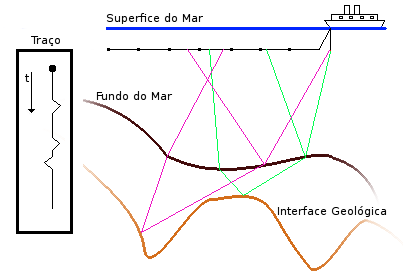
\includegraphics[scale=.7]{navio.png}}
	\caption{Coleta de dados em levantamento sísmico marítimo.}
	\label{fig:sim}
\end{figure}

\subsection{Avaliação e Otimização de Desempenho}

Os resultados apresentados nessa seção foram medidos no sistema \emph{draco} do Grupo de Processamento Paralelo e Distribuído\footnote{\url{http://gppd-hpc.inf.ufrgs.br/}} (GPPD) da Universidade Federal do Rio Grande do Sul (UFRGS). Cada nó da \emph{draco} consiste de 2 processadores Intel Xeon E5-2630 de 8 núcleos, totalizando 16 \textit{threads (Hyper-Threading)}, além de 64 GB DDR4.

Nessa atividade, o objetivo é implementar uma versão paralela e vetorial otimizada da aplicação de Geofísica. O primeiro passo é verificar o desempenho da \textit{cache}, buscando após, encontrar um dos laços para vetorizar. Utilizando o comando: 

\begin{lstlisting}[frame=none, numbers=none]
@\textcolor{mygreen}{\$ perf stat -e cache-misses,cache-references src/6-kernel.exec}@
\end{lstlisting}

verifica-se a taxa de acerto de \textit{cache} da versão original. A taxa retornada nesse caso foi de 27\%, sendo que essa é considerada baixa. Buscando melhorar o desempenho da aplicação, otimizando os acessos a \textit{cache}, utilizou-se a técnica de \textit{loop interchange} para alterar a ordem dos laços. A taxa de acerto para diferentes combinações pode ser vista na Tabela~\ref{tab:oil:cache}. Uma vez que a ordem \texttt{k, Y, X} obteve a maior taxa de acerto, continuou-se com essa, agora buscando efetuar a vetorização.

\begin{table}[!htb]
    \centering
    \caption{Taxa de Acerto da Aplicação Geofísica}
    \label{tab:oil:cache}
    \begin{tabular}{cc}
        \toprule
        Ordem dos laços     & Taxa de Acerto (\%)                 \\ \midrule
        \texttt{X, Y, k}  & 26.9\% \\
        \texttt{Y, k, X}  & 93.6\% \\
        \texttt{k, Y, X}  & 95.8\% \\ \bottomrule
    \end{tabular}
\end{table}

No caso da vetorização, identificou-se que o laço mais interno pode ser vetorizado. Isso é possível, pois a maior parte dos acessos à memória é feita de forma contígua em direção aos pontos em X. O perf também pode ser utilizado para analisar o uso de instruções SIMD via comando: 

\begin{lstlisting}[frame=none, numbers=none]
@\textcolor{mygreen}{\$ perf stat -e simd\_fp\_256.packed\_single,simd\_fp\_256.packed\_double src/6-kernel.exec}@
\end{lstlisting}

verificou-se que após adicionar a diretiva \texttt{omp simd}, o número de instruções \texttt{simd} de precisão simples mudaram de $0$ para $3 429 629 397$. 

Por fim, a Tabela~\ref{tab:results} apresenta os resultados de tempo de execução das diferentes versões utilizando como entrada um cubo de tamanho 512. A versão na qual melhorou-se o desempenho da \textit{cache} foi 5,2$\times$ mais rápida que a versão sequencial. A versão vetorial utilizando unidades vetoriais melhorou o desempenho da aplicação em 3,6$\times$ em relação a versão com \textit{cache} otimizada. A versão paralela em OpenMP foi executada com 32 \textit{threads}, melhorando o desempenho da aplicação em 4,1$\times$. A versão final, que combina todas otimizações, teve o melhor desempenho, de 75,5$\times$ em relação a versão sequencial. Essas e outras propostas de otimização para essa aplicação de geofísica podem ser vistas em diversos trabalhos~\cite{serpa2017strategies, serpa2018optimizing, serpa2018improving, serpa2019optimization}.

\begin{table}[!htb]
\centering
\caption{Desempenho da Aplicação Geofísica}
\label{tab:results}
\begin{tabular}{cc}
\toprule
Versão     & Tempo de Execução (s)   \\ \midrule
Sequencial & 90,6                    \\ 
Cache      & 17,5                    \\ 
Vetorizada &  4,9                    \\ 
OpenMP     &  1,2                    \\ \bottomrule
\end{tabular}
\end{table}
\section{Conclusão} \label{sec:conclusion}

O uso de arquiteturas paralelas e vetoriais é uma solução para incrementar a capacidade de execução, tornando possível a computação eficiente de aplicações com grande demanda de processamento. Para tanto, é preciso fazer uso de interfaces de programação paralela. Neste capítulo foram apresentados detalhes da interface \emph{OpenMP}, a qual é amplamente utilizada em aplicações de alto desempenho para ambientes de memória compartilhada. Com isso, é possível criar aplicações com múltiplas \emph{threads} de forma prática. Desta forma, é possível a solução eficiente de problemas que possuem algum tipo de concorrência. 

Além disso, mostrou-se como utilizar as ferramentas perf e PAPI para analisar o desempenho de aplicações paralelas. Essas ferramentas leem contadores de \textit{hardware} do processador e auxiliam no entendimento de otimizações propostas. Desta forma, como mostrado no estudo de caso de uma aplicação geofísica, é possível maximizar o uso dos recursos computacionais disponíveis nas arquiteturas atuais, com isso, melhorando o desempenho de aplicações sintéticas e reais.

No futuro, planeja-se abordar outras interfaces de programação paralela como Intel TBB, MPI, CUDA, entre outras.

Exercícios e soluções deste capítulo estão disponíveis em:

\url{https://gitlab.com/msserpa/prog-paralela-erad}.


\bibliography{referencias}

\end{document}
